\subsection{MDL of a Zero-Dimensional Manifold Cluster}
\label{ssc:zero-dim-mdl}




An interesting case arises when we try to calculate the MDL of
a zero-dimensional manifold cluster. Given that a zero-dimensional (ZD)
manifold is a point, any cluster characterized only by its center point is
considered as a zero-dimensional manifold or spherical cluster
\IfClass{IEEEtran}{}{, see Fig.~\ref{fig:zdc}}.
Many clustering algorithms, e.g. $k$-means, produce zero-dimensional manifold
clusters \cite{Jain:1999mf}.

\ifIEEEtran
\else
\begin{figure}[ht]
\center
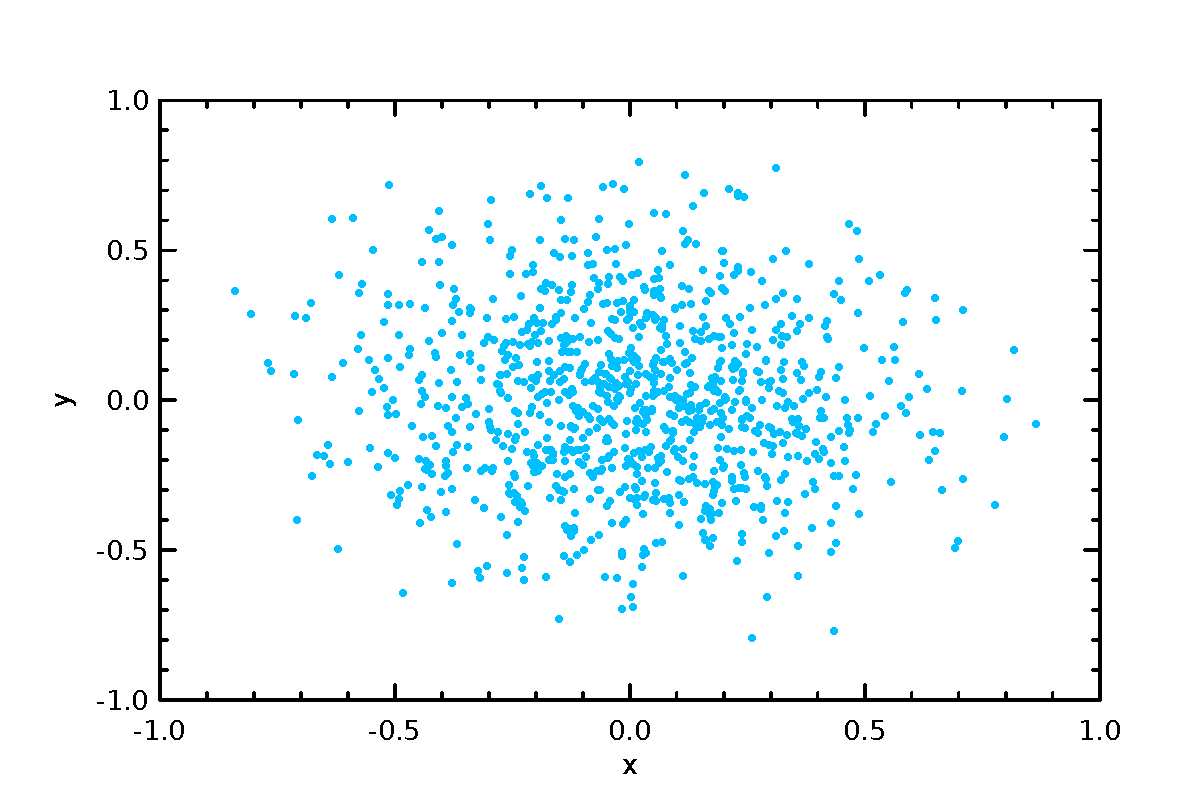
\includegraphics[width=3.5in]{img/zero-dim-mdl_zdc_1.pdf}
\caption{Spherical (zero-dimensional linear manifold) cluster in 2D space}
\label{fig:zdc}
\end{figure}


\fi

Any zero-dimensional manifold cluster is a special case of the linear manifold
cluster, thus we can use encoding (\ref{eq:mdl-lmc-final}) to calculate the MDL
value of the cluster given that dimension of the manifold is zero, $M = 0$.
Thus, (\ref{eq:mdl-lmc-final}) is simplified as follows
\begin{equation} \label{eq:mdl-zdm}
L(\varepsilon) = P_m N + J S(\varepsilon)
\end{equation}

Georgieva et al. \cite{Georgieva:2011tk} took a similar approach in
describing the MDL of zero-dimensional clusters, produced by the $k$-means
algorithm. However, instead of using the entropy of the quantized distribution
of the point positions in particular dimensions, the projection distances to
the point were encoded in MDL as follows
\begin{equation} \label{eq:mdl-zdc}
L = L(H) + L(D|H) = P N + \sum_{i=1}^{J} \sum_{p=1}^{N} \log (d_i^p + 1)
\end{equation}
where $d_i^p$ corresponds to the projection of the distance $d_i$ of
the $i$-th point to the $p$-th dimension.
Such a description does not provide an informative encoding of coordinates when
distances to the center in the cluster are near zero. In such a case, distance
is encoded with less than one bit on the average.

We will compare the degenerate case of the inexact encoding of zero-dimensional
manifold cluster calculated by (\ref{eq:mdl-zdm}) on synthetically generated
linear manifold and spherical clusters. Such an approach will provide a common
ground for comparison between linear manifold and spherical clusters.
We also compare the MDL value of a linear manifold clustering with a cumulative
MDL of a clustering constructed from zero-dimensional clusters which is a more
natural representation of linearly shaped data from the perspective of spherical
clustering algorithms.

% Use 1D manifold (as above) for 0D MDL calculation under various quantization errors.
We used a synthetically generated dataset which has a form of a 1D linear manifold
cluster, an elongated dataset along the one axis, in 2D full space.
Cluster generation procedure was described above.
%described in the section \ref{sc:results}.
We performed the MDL value calculation for the 1D manifold following MDL formula
\eqref{eq:mdl-lmc-final} and then the 0D manifold case defined by \eqref{eq:mdl-zdm}
for various quantization errors.

\begin{figure}[ht]
\center
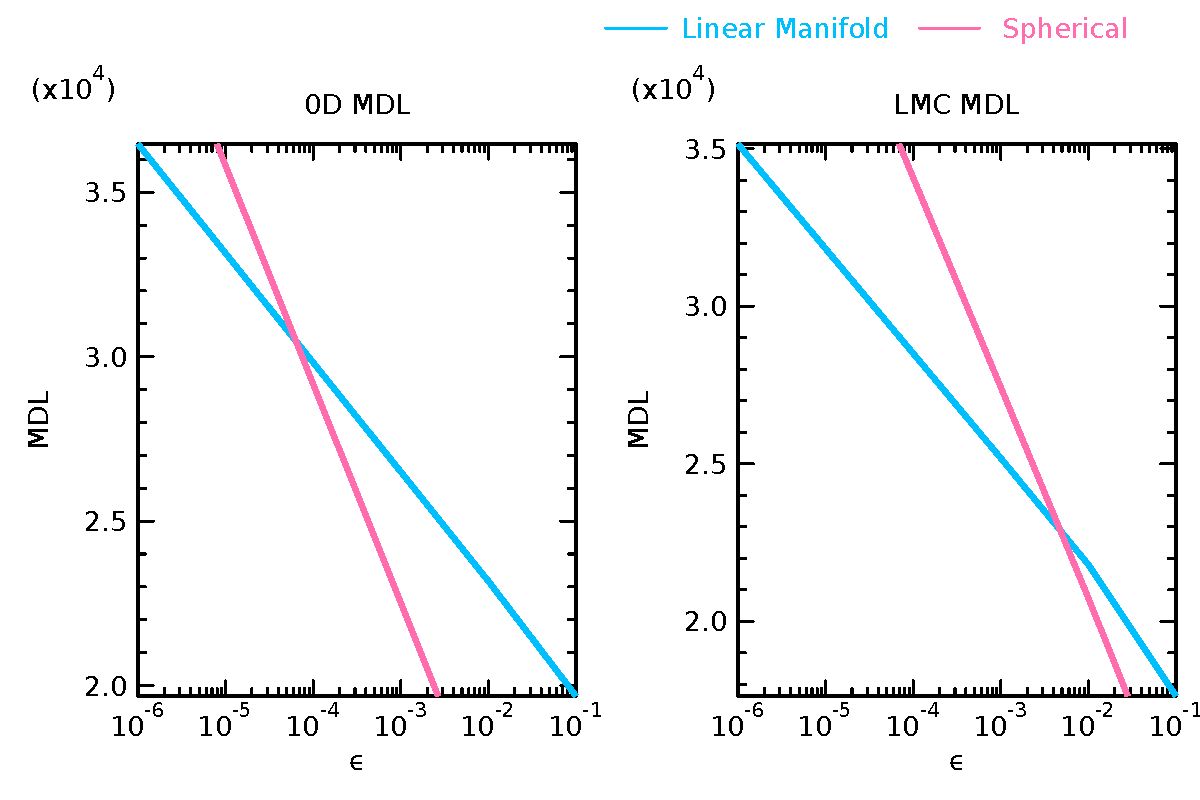
\includegraphics[width=3.5in]{img/zero-dim-mdl_zdc-mdl-exp1_1.pdf}
\caption{Linear manifold (1D) and zero-dimensional (0D) MDL calculations for 1D linear manifold and spherical 0D clusters, located in 2D space, with various quantization errors \textepsilon.}
\label{fig:zdc-mdl-exp1}
\end{figure}



Figure~\ref{fig:zdc-mdl-exp1} shows results of linear manifold Eq.~\eqref{eq:mdl-lmc-final}
and zero-dimensional Eq.~\eqref{eq:mdl-zdm} MDL value calculations for various types
of manifold clusters. For large quantization errors, both approaches to the MDL
calculation produce a small MDL value for spherical cluster. However, when
the precision of the quantization procedure increases, resulting in a more
complete and informative description of the cluster, the MDL value of the linear
manifold cluster becomes smaller than the spherical cluster regardless of
the selected method of calculation.
% Although, LM-MDL approach provides smaller value of the linear
% manifold cluster under the larger quantization error, then ZD-MDL approach.
\IfClass{IEEEtran}{}{\bigskip}

%Use k-means to cluster 1D linear manifold, k>=1, and calculate total MDL of clustering. Compare resulted value to the MDL of 1D LM.

Because of the structural difference between linear manifold and spherical
clusters, it is hard to come with common criteria for comparison of
different types of clusters. We use the MDL value as a measure for
heterogeneous cluster comparison. In order to test how the cluster MDL would
perform as a comparison score, we calculated MDL values of synthetically
generated clusters of different types - linear manifold and spherical.

We generated a 1D linear manifold cluster dataset from a bivariate normal
distribution, as in previous experiments, and used the $k$-means algorithm to
synthesize spherical clusters from it. We varied the number of clusters for
the $k$-means algorithm that allowed us to form clusters which gradually
obtain a spherical shape, as the linear manifold cluster got partitioned
into more clusters.

We perform an evaluation of the MDL value for the linear manifold clusters by
Eq.~\eqref{eq:mdl-lmc-final} and spherical cluster by Eq.~\eqref{eq:mdl-zdm}.
When $k$-means generated more than one cluster from the original dataset,
we summed all the cluster MDL values in the clustering to obtain
the MDL score for the original 1D LM cluster represented by the dataset.
\IfClass{IEEEtran}{This is shown in Figure~\ref{fig:mdl-zdc-exp2}.}{}

\begin{figure}[ht]
\center
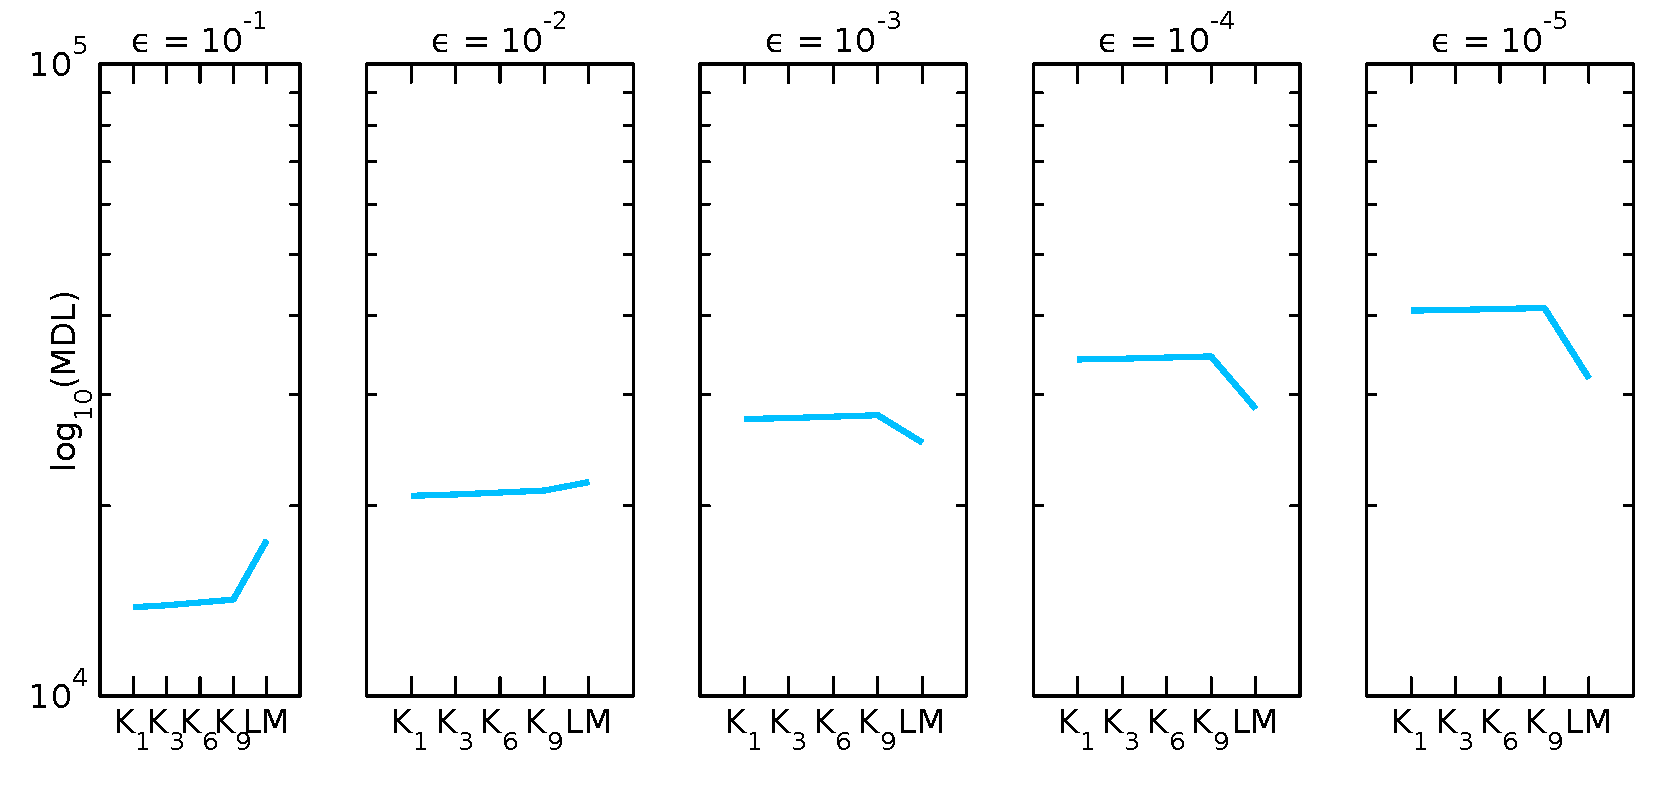
\includegraphics[width=3.5in]{img/zero-dim-mdl_zdc-mdl-exp2_1.pdf}
\caption{MDL value of k-means clusterings (K[k]) produced from the 1D linear manifold cluster (LM), located in 2D space, under various quantization errors \textepsilon.}
\label{fig:zdc-mdl-exp2}
\end{figure}



\IfClass{IEEEtran}{}{
Figure \ref{fig:mdl-zdc-exp2} shows results of MDL calculations for clusterings
produced from the 1D linear manifold cluster.}We found that the division of
the linear manifold on multiple spherical clusters does not provide much
difference in the resulted MDL value. As in the previous experiment, the major
factor which affects MDL calculations is the quantization error parameter.
For a small quantization error, spherical clusters provide a smaller MDL value
for the experimental dataset. Moreover, the MDL value of the whole dataset does not
increase significantly with the number of clusters in the $k$-means clustering.
However, as the quantization error decreases, the MDL value calculated by
Eq.~\eqref{eq:mdl-lmc-final} becomes significantly smaller then the spherical
cluster MDL value Eq.~\eqref{eq:mdl-zdm}.

This result suggests that for a large quantization error a spherical description
of the linear manifold cluster provides more compact MDL value over
the linear manifold MDL model. But while the quantization error decreases,
giving a better description of the data, the linear manifold MDL model produces
more compact encoding of the linear manifold cluster and outperforms the spherical
MDL model regardless of cluster proximity to true spherical representation.
